\subsubsection{MLP}

To construct the MLP, RoBERTa-generated embeddings were initially loaded. The dataset was then partitioned into training and testing subsets, with an 80/20 split, respectively.

The primary consideration in designing the MLP architecture was determining the optimal number of dense layers and neurons. To this end, a manual cross-validation procedure was conducted to evaluate different architectural configurations. The hyperparameters explored included the number of hidden layers (1, 2, or 3) and the number of neurons in the first hidden layer (32, 64, or 128).

For architectures with more than one hidden layer, each subsequent layer contained half the number of neurons of its preceding layer. Based on validation performance, the best configuration consisted of two hidden layers: the first with 32 neurons and the second with 16 neurons, as illustrated in Figure~\ref{fig:mpl_layer_diagram}.


\begin{figure}[htbp]
    \centering
    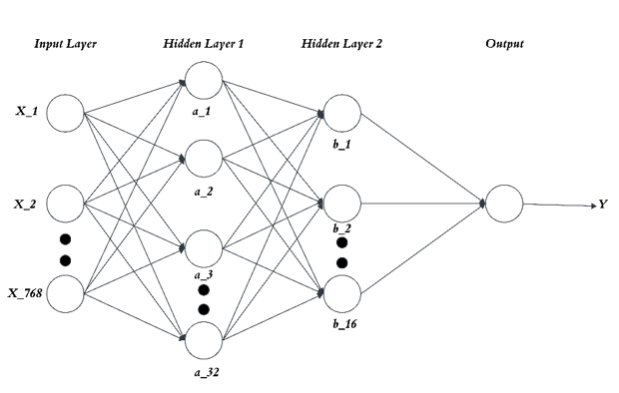
\includegraphics[width=0.8\linewidth]{images/MPL_layer_diagram.png}
    \caption{Diagram of the MLP layer architecture.}
    \label{fig:mpl_layer_diagram}
\end{figure}
